
\begin{center}
\Huge
Regressioner og regressionsanalyse
\end{center}
\section*{Regression}
\stepcounter{section}
Vi skal i dag se på regressionsanalyse.

\begin{exa}
Vi betragter datapunkterne fra \href{https://github.com/ChristianJLex/TeachingNotes/raw/master/2023-2024/Data og lign/regression_eksempel.xlsx}{\color{blue!60} dette datasæt}.
Vi ved ikke, hvilken underlæggende sammenhæng, der skaber dataet, kan vi prøve at lave forskellige regressioner på det. Dette gøres i Maple og kan ses af Fig. \ref{fig:regression}

\begin{figure}[H]
\centering
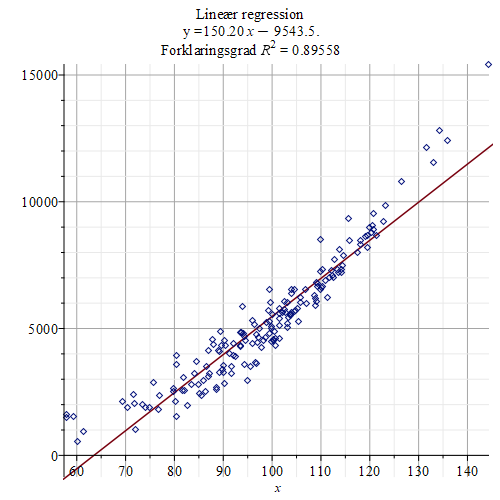
\includegraphics[width = \textwidth*4/10]{Billeder/LinRegtilRes.png}
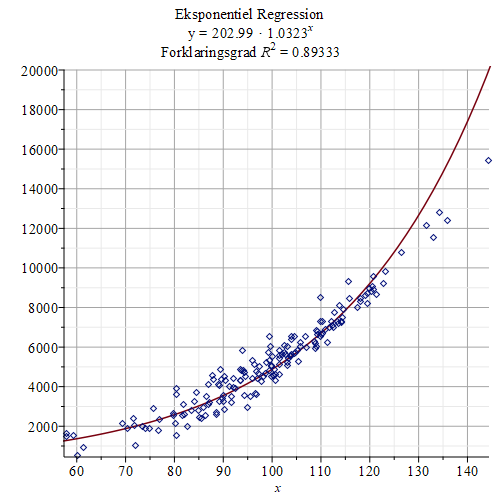
\includegraphics[width = \textwidth*4/10]{Billeder/ExpRegtilRes.png}
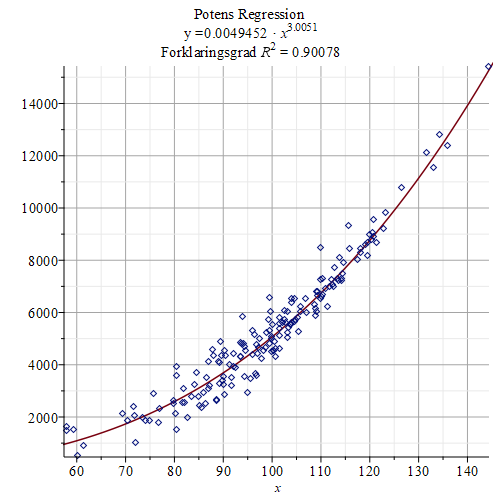
\includegraphics[width = \textwidth*4/10]{Billeder/PowRegtilRes.png}
\caption{Lineær regression, eksponentiel regression og potensregression på datasæt}
\label{fig:regression}
\end{figure}
Hvordan afgør vi så, hvilken af modellerne der er bedst, hvis vi ikke har yderligere information omkring kilden af dataet? Man kan ikke sammenligne korrelationskoefficienter mellem modeller. Derfor skal vi lave regressionsanalyse. En del af regressionsanalyse er blot at betragte de fittede modeller og se, hvilken model der ser ud til at passe bedst. I dette tilfælde ser det ud til at være potensmodellen. 
\end{exa}


\section*{Regressionsanalyse}

Til at vurdere, om en regression er god, skal vi bruge et værktøj til at afgøre, om det modellen rammer forbi blot er tilfældige fejl eller om vi rammer strukturelt forkert. Første tilfælde er ønskværdigt. Vi definerer nu residualerne til en regression.
\begin{defn}
Givet måledata $(x_1,y_1),(x_2,y_2),\hdots,(x_n,y_n)$ og regressionsmodel $f(x)$, så definerer vi det $i$'te residual som det, modellen $f$ rammer forbi den målte værdi. Mere præcist
\begin{align*}
r_i = y_i - f(x_i).
\end{align*} 
\end{defn}
Det er klart, at en god model $f(x)$ vil have små residualer. Udover dette så vil vi også have normalfordelte residualer. Det vil sige, at vi gerne vil have mange residualer tæt på 0 og kun få langt fra 0. Der må ikke være nogen yderligere struktur i residualerne. For at se, hvad dette betyder, ser vi på et eksempel.

\begin{exa}
Betragter vi regressionerne fra tidligere eksempel, kan vi finde residualerne for de tre modeller. Disse findes i Maple ved eksempelvis
\begin{align*}
	\texttt{plotResidualer(X,Y,LinReg)} 
\end{align*}
 i fald residualerne skal findes for lineær regression. Residualerne for de tre modeller kan ses af Fig. \ref{fig:resplot}
\begin{figure}[H]
\centering
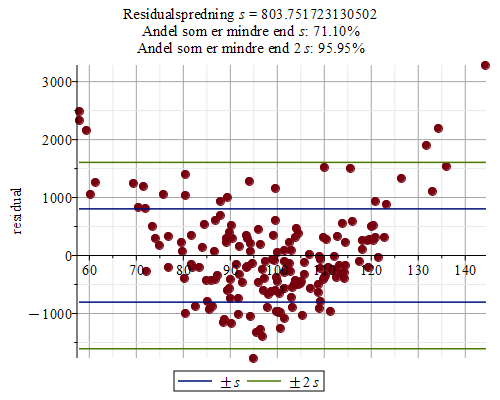
\includegraphics[width = \textwidth*4/10]{Billeder/LinRegResidual.png}
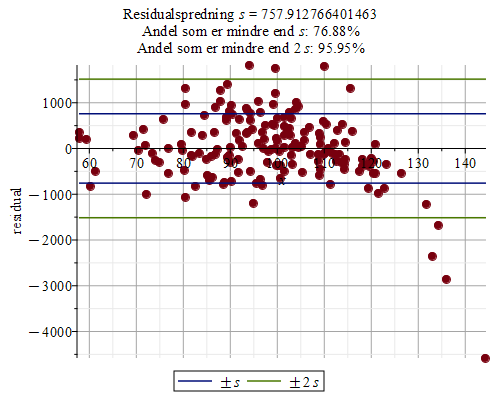
\includegraphics[width = \textwidth*4/10]{Billeder/ExpRegResidual.png}
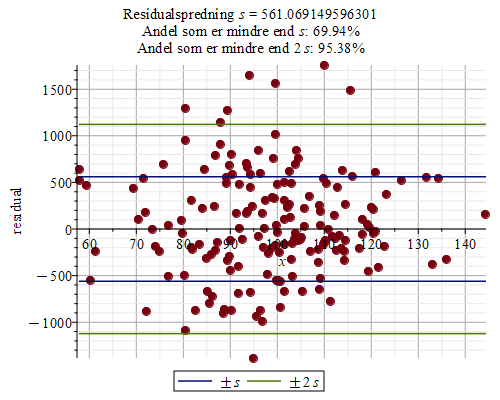
\includegraphics[width = \textwidth*4/10]{Billeder/PowRegResidual.png}
\caption{Lineær regression, eksponentiel regression og potensregression på datasæt}
\label{fig:resplot}
\end{figure}
	Vi ønsker at se et tilfældigt mønster i residualerne, og derfor ser det ud til at 
	potensregressionen beskriver datapunkterne bedst
\end{exa}
\subsection*{Opgave 1}
\stepcounter{section}

Lav regression på følgende datasæt og afgør med residualanalyse hvilken model der passer bedst.
\begin{center}
\begin{tabular}{c|c|c|c|c|c|c|c|c|c}
1 & 2 & 3 & 4 & 5 & 6 & 7 & 8 & 9 & 10\\ \hline
1.45 & 14.96 & 7.22 & 26.63 & 45.49 & 66.88 & 103.90&157.63 & 162.63 & 252.61
\end{tabular}
\end{center}

\subsection*{Opgave 2}

I \href{https://github.com/ChristianJLex/TeachingNotes/raw/master/2023-2024/Data%20og%20lign/bakterierResidual.xlsx}{\color{blue!60} dette datasæt} findes antal bakterier i mia. sammenholdt med den forløbne tid i timer i en bestemt bakteriekoloni. 

\begin{enumerate}[label=\roman*)]
	\item Afgør, hvilken regressionstype, der passer bedst på datasættet ved at bruge 
	residualerne for modellen.
	\item Brug din valgte model til at bestemme, hvor mange bakterier der vil være efter 30 
	timer.
\end{enumerate}

\subsection*{Opgave 3}

I \href{https://github.com/ChristianJLex/TeachingNotes/raw/master/2023-2024/Data%20og%20lign/beboereResidual.xlsx}{\color{blue!60} dette datasæt} findes antal beboere i en by angivet efter antal forløbne år efter år 1900.

\begin{enumerate}[label=\roman*)]
	\item Afgør, hvilken regressionstype, der passer bedst på datasættet ved at bruge 
	residualerne for modellen.
	\item I hvilket år vil der i følge din model være 8000 beboere i byen?
\end{enumerate}

\subsection*{Opgave 4}

I \href{https://github.com/ChristianJLex/TeachingNotes/raw/master/2023-2024/Data og lign/Baevervaegt.xlsx}{\color{blue!60} dette datasæt} fremgår længden i cm og vægten i kg af 122 europæiske bævere. 

\begin{enumerate}[label=\roman*)]
	\item Afgør, hvilken regressionstype, der passer bedst på datasættet ved at bruge 
	residualerne for modellen.
	\item Hvor lang skal en bæver ifølge modellen være for at veje 25kg?
\end{enumerate}

\subsection*{Opgave 5}

I \href{https://github.com/ChristianJLex/TeachingNotes/raw/master/2023-2024/Data og lign/Chokoladepris.xlsx}{\color{blue!60} dette datasæt} fremgår sammenhængen mellem prisen på en bestem plade chokolade og antal passerede år efter år 1990.

\begin{enumerate}[label=\roman*)]
	\item Afgør, hvilken regressionstype, der passer bedst på datasættet ved at bruge 
	residualerne for modellen.
	\item Hvad er prisen på en plade chokolade i år 2010 ifølge modellen?
\end{enumerate}

\subsection*{Opgave 6}

I \href{https://github.com/ChristianJLex/TeachingNotes/raw/master/2023-2024/Data og lign/Laegemiddel.xlsx}{\color{blue!60} dette datasæt} fremgår koncentrationen i blodet (i mg/L) af et bestemt lægemiddel og antal forløbne timer efter indtagelsen.

\begin{enumerate}[label=\roman*)]
	\item Afgør, hvilken regressionstype, der passer bedst på datasættet ved at bruge 
	residualerne for modellen.
	\item Hvornår er koncentrationen i blodet under 0.5mg/L?
\end{enumerate}